\section{Module 1 - Data Collection}
\par Like in any other system that deals with data processing, the prime component of the market intelligent system is the data. Data here refers to the information regarding the concerned companies and products that are gathered though various means.\\
Data collection for the system is done in two phases
\begin{itemize}
\item Initial Database Creation
\item Dynamic Data Collection
\end{itemize}
\subsection{Initial Database Creation}
\par To start with, we need to accumulate details regarding existing companies, their products and other relevant information. Working on an area like Technology, we are particularly interested in the following kinds of details regarding a company.
\begin{itemize}
\item Registered name
\item Launched products
\item Locations 
\item Associated and relevant people
\item Website information
\item Contact information
\item Acquisition details
\end{itemize}
\par Initial Database creation is a one-time process in the entire lifecycle of the system. It is meant to provide an initial database platform for the dynamic data updation procedure that follows. The data collection is done through various API modules available.

\subsubsection{Collecting Company Names}
\paragraph*{Clearbit’s Discovery API v1.0}
\hfill \break 
The first and foremost step is to make a list of companies working in the field that we are concerned with. The Discover API by Clearbit is used for this purpose. It helps to create a targeted list of companies using an advanced search parameter. The main 	features behind the selection of Discovery API for the purpose are.	

\begin{itemize}
\item Flexible API \\ Create lists of prospects for internal use or integrate the API directly into the system
\item Fast \\ It is considered to be relatively fast and light weighed when compared to counter options.
\item Reliable and Growing database. \\The database is constantly growing, up-to-date and is reliable.
\end{itemize}
\paragraph*{API invocation format}
\hfill
\par The calls to the API module are done as rest calls, passing the field of interest as the parameter.
\paragraph*{API response format}
\hfill \break
The response to the rest call is received in json format and need to be parsed to obtain individual company names.
\begin{figure}[h]
	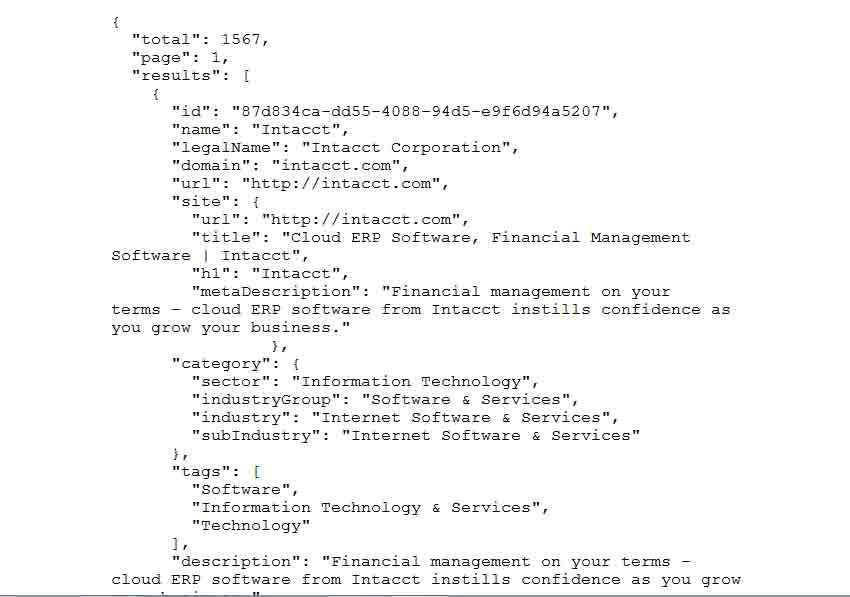
\includegraphics[width=15cm, height=12cm]{discovery1}
	\centering
	\caption{Response format of Discovery API Part1}
\end{figure}
\begin{figure}[h]
	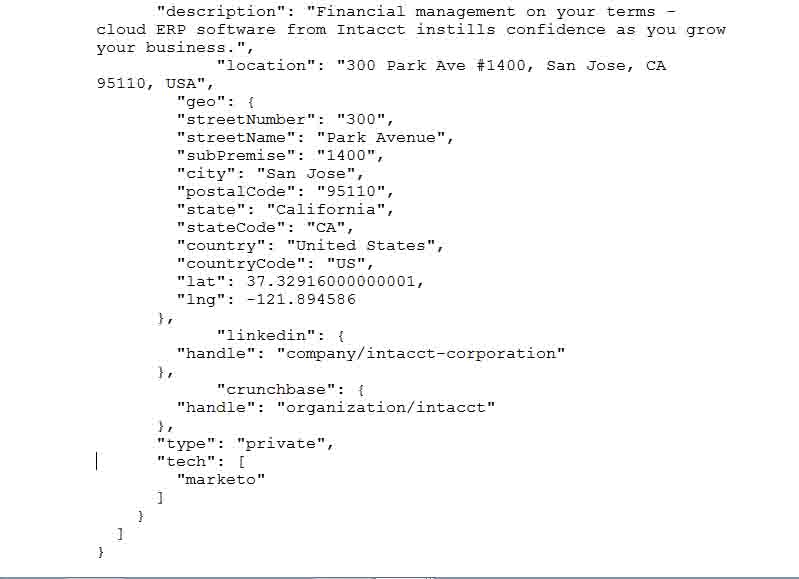
\includegraphics[width=15cm, height=12cm]{discovery2}
	\centering
	\caption{Response format of Discovery API Part2}
\end{figure}
\subsubsection{Collecting Company Details}
\paragraph*{CrunchBase API v2.0}
\hfill \break
The CrunchBase API gives developers, access to query the CrunchBase Dataset for both paginated lists of specific types of Items (e.g., Companies) and details about individual Items (e.g., the properties and relationships of a specific Company).
Developers can navigate through the Dataset by retrieving and inspecting individual Items and their relationships. Each detailed Item response includes not only the properties of the Item (e.g., a Company's name, founding date, and profile image) but also a list of all of its relationship types (e.g.,"competitors","current team").\cite{clearbit}
\paragraph*{API invocation format}
\hfill \break
The calls to the API module are done as rest calls, passing the company name as the parameter.
\paragraph*{API response format}
\hfill \break
The response to the rest call is received in json format and need to be parsed to obtain tabulated details of each company.
\begin{figure}[h]
	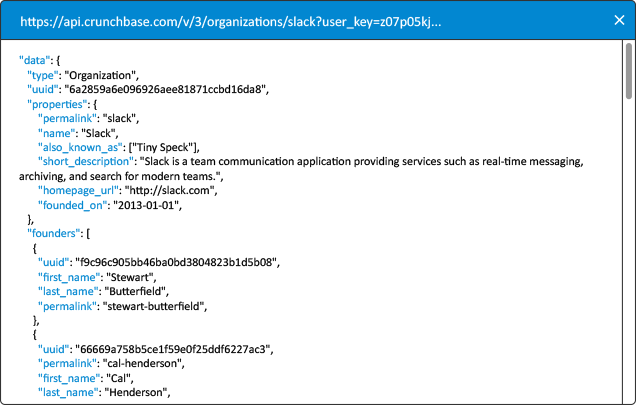
\includegraphics[width=12cm, height=8cm]{crunchbase}
	\centering
	\caption{response format of CrunchBase API}
\end{figure}
\par
The API allows only a limited number of calls to be made per account holder per hour. Hence the calls need to done as a scheduled task considering this limitation. Also, the process of retrieving the individual company details using the API might take a time delay of approximately two seconds per call. As a result, making calls in a sequential manner isn’t the best of options. This limitation is overcome by the application of multithreaded approach to API calls where concurrent calls and made at a time, collecting information regarding different companies.
\begin{figure}[h]
	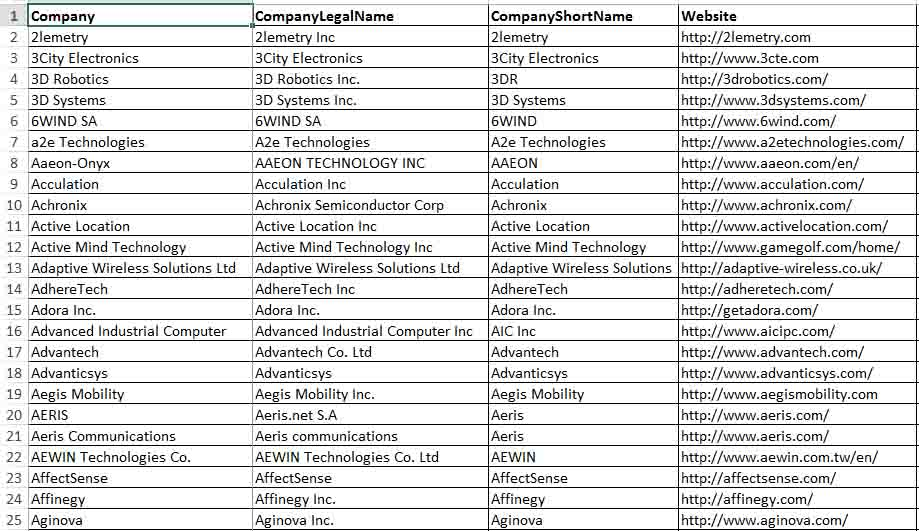
\includegraphics[width=15cm, height=10cm]{initial_db1}
	\centering
	\caption{Miniature tabulated format of details collected - part 1}
\end{figure}
\begin{figure}[h]	
	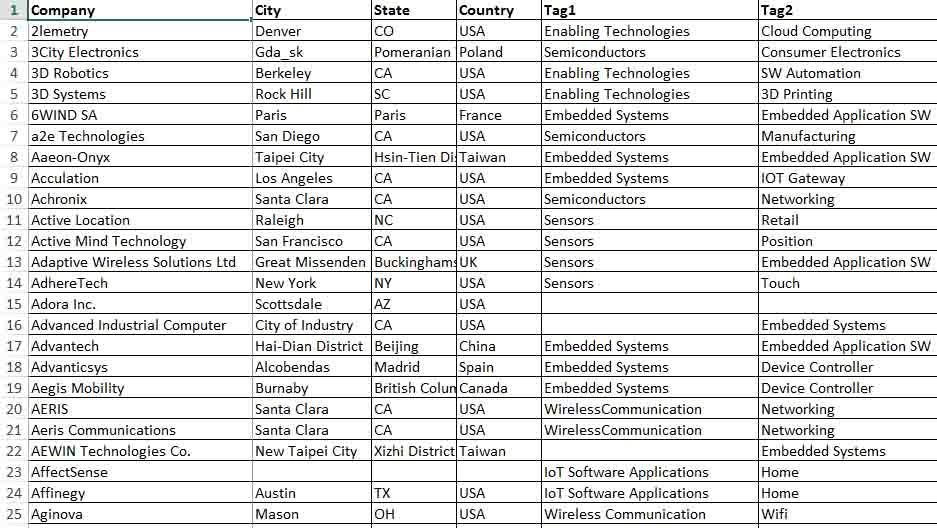
\includegraphics[width=15cm, height=10cm]{initial_db2}
	\centering
	\caption{Miniature tabulated format of details collected - part 2}
\end{figure}

\subsection{Dynamic Data Collection}
\par Once the initial database is created, it is required to make dynamic updation of data in order to incorporate the latest trends and happenings in the area (eg: Technology) concerned. This is done by extracting the relationships from articles and data made available from RSS feeds. The selection of reliable and consistent RSS feeds is done by the administrator. The extraction of details provided by the feeds is done by ROME API.
\subsubsection{Extraction from RSS feeds}
\paragraph*{ROME API}
\hfill \break
Rome is based around an idealized and abstract model of a Newsfeed or "Syndication Feed". Rome can parse any format of Newsfeed, including RSS variants and Atom, into this model. Rome can convert from model representation to any of the same Newsfeed output formats. Here we use the API module to parse the response provided by the feed in XML/Atom format.\cite{romeapidocs}

\paragraph*{API invocation format}
\hfill
\par The calls to the API module is done by passing the xml/atom file to the module.
\paragraph*{API response format}
\hfill \break
The API responds by providing an object that contains the parsed details of the concerned field. This contains the URLs to the articles as well as their short titles.
\begin{figure}[h]
	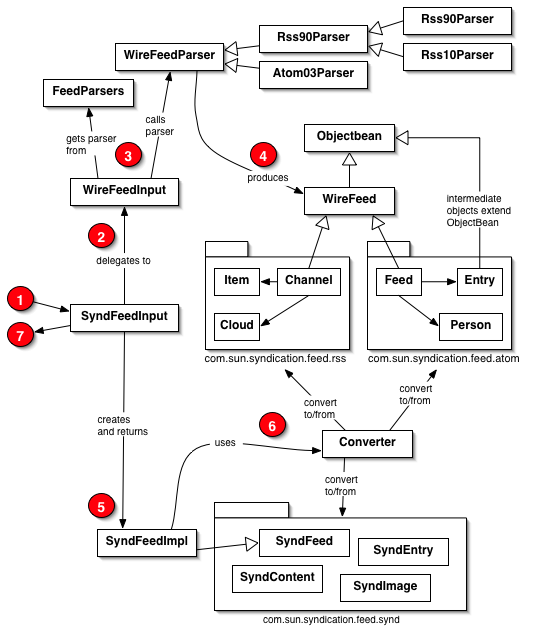
\includegraphics[width=10cm, height=11cm]{HowRomeWorks}
	\centering
	\caption{Internal working diagram of ROME API}
\end{figure}
\par When we are done collecting the URLs for the articles, the next step is to retrieve the text articles from the concerned URLs. 

\subsubsection{Extracting article text}
\paragraph*{Boilerpipe API}
\hfill \break
The URLs to articles return a page containing the concerned article as well as other elements such as advertisements, hyperlinks to other pages, promotional details etc. For the extracted data to be of some value, it is needed to retrieve only the potential article text from the URL and Boiler pipe API serves this need.
\paragraph*{API invocation format}
\hfill
\par The calls to the API module is done by passing the concerned URL to the module.
\paragraph*{API response format}
\hfill \break
The API responds by providing an object that encapsulates the article details and can be used to retrieve the text article for further processing.
\begin{figure}[h]
	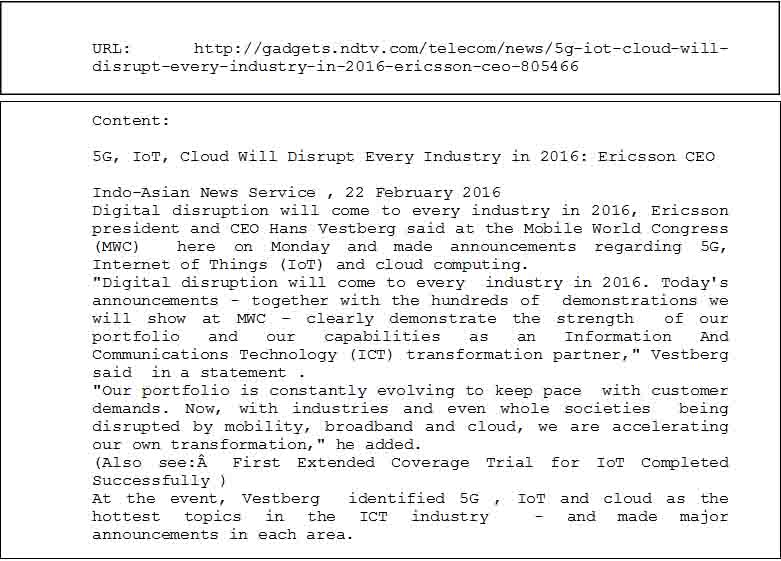
\includegraphics[width=10cm, height=8cm]{boilerpipe}
	\centering
	\caption{An example of passed URL and extracted text by Boilerpipe API}
\end{figure}

\section{Module 2 - Data Processing}
\par
For the retrieved articles to be incorporated to the existing database, it is needed to derive possible relations out of the articles and tag them accordingly. Data processing phase is aimed at providing this service. 
\paragraph*{Input to the phase:}
The article in text format is served as input to the data processing phase.
\paragraph*{Output from the phase:}
Consistent relationships involving concerned companies, products and their relationships are derived in the form of triplets (subject, object, verb).

\subsection{Initiating Context vocabulary}
\par The administrator need to establish a table with all the possible verb terms we are interested in the relation and those which are expected to be identified by the API module. This is to identify the context of each article and categorize them accordingly.
\\ A minimized list of contexts can be identified as 
\begin{itemize}
\item Tech Invest	
\item R\&D	
\item New Product Introduction	
\item Executive Moves	
\item Outsourcing And Offshoring	
\item Contracts Central	
\item Technology In Action	
\item Intellectual Property Rights	
\item Talent Tracker
\item M\&A Tracker
\end{itemize}

\subsection{Initiating Taxonomy vocabulary}
\par It is also required to maintain a table containing the taxonomy terms we are interested in. This is to relate the keywords extracted by the API with each taxonomy terms and tag articles accordingly.
\\
A minimized list of taxonomies can be identified as
\begin{itemize}
\item Social Networks
\item Social Media
\item Social Trends	
\item Social Challenges	
\item Mobile Devices	
\item Mobile Networks	
\item IoT	
\item Mobile Apps
\item Big Data	
\item Business Analytics	
\item Location Analytics	
\item Information Management	
\item Cloud Infrastructure	
\item Cloud Computing	
\item Saas/PaaS/IaaS	
\item Virtualization
\end{itemize}

\subsection{Defining Grammars}
\par To make the system work efficiently in identifying relations, the administrator need to define various grammars characterizing the relations the system is intended to accommodate. Once a relation is retrieved by the API, it is compared with the grammar syntaxes to validate the relevance of the relation. Only those relations that match some grammar syntax will be validated and added to the database. This is a very important phase of the entire system since the efficiency with which the system will work depends heavily on the efficiency with which grammars are formulated.
\\
Examples for grammars involving companies and products in Technology field may be identified as
\begin{itemize}
\item Company Acquires Company.
\item Company Launches Product.
\item Company Invest in Technology.
\end{itemize}

\subsection{Extracting Relations from articles}

\paragraph*{AlchemyAPI}
\hfill \break
AlchemyAPI uses natural language processing technology and machine learning 	algorithms to extract semantic meta-data from content, such as information on people, 	places, companies, topics, facts, relationships, authors, and languages. AlchemyAPI 	provides easy-to-use mechanisms to identify positive/negative sentiment within any 	document or web page. AlchemyAPI Sentiment Analysis APIs are capable of computing 	document-level sentiment, user-specified sentiment targeting, entity-level sentiment, 	emoticons and keyword-level sentiment. Multiple modes of sentiment analysis provide 	for a variety of use cases ranging from social media monitoring to trend analysis. In our system, we are particularly interested in using AlchemyAPI to retrieve keywords and relations from the input articles.\cite{alchemy-relation}

\paragraph*{API invocation format}
\hfill
\par The calls to the API module is done by passing the article text to the API.
\paragraph*{API response format}
\hfill \break
The API responds by providing an object that encapsulates the keywords and relations 	extracted from the article.
\begin{figure}[h]
	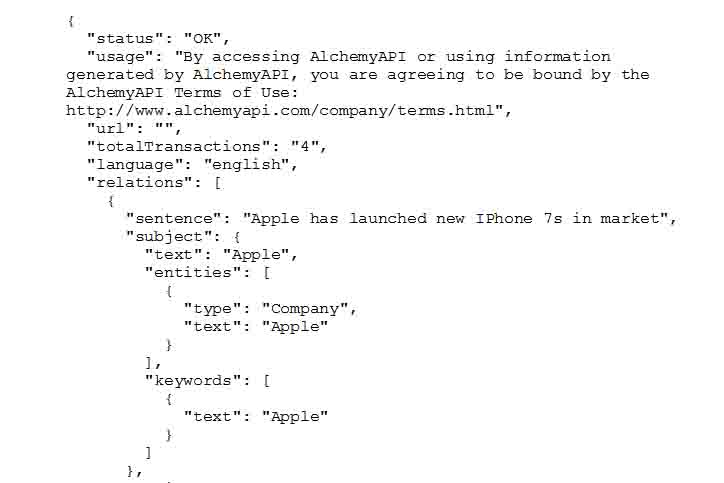
\includegraphics[width=13cm, height=9cm]{alchemy1}
	\centering
	\caption{An example of response format by Alchemy API Part1}
\end{figure}
\begin{figure}[h]
	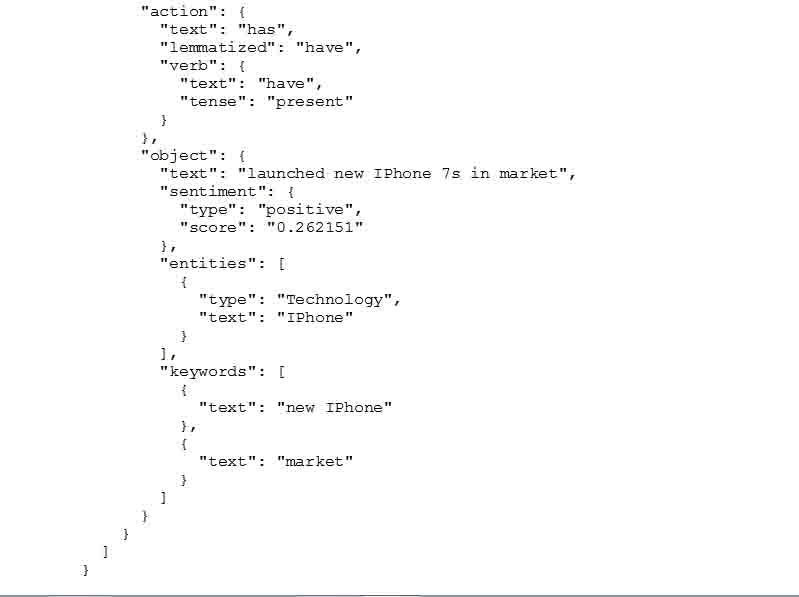
\includegraphics[width=13cm, height=9cm]{alchemy2}
	\centering
	\caption{An example of response format by Alchemy API Part2}
\end{figure}
\par 
The relations extracted from the article will be available in the form of triplets. It will be 	of the form \\(SUBJECT, OBJECT, VERB)
\begin{figure}[h]
	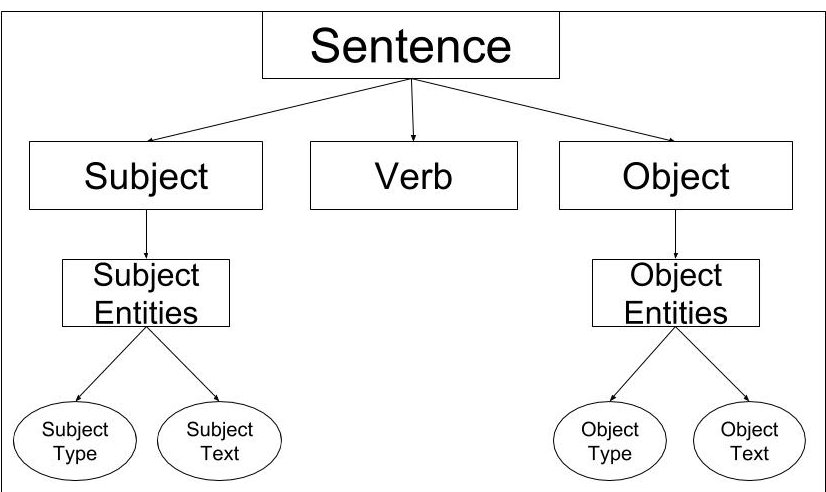
\includegraphics[width=13cm, height=7cm]{sentenceDiagram}
	\centering
	\caption{Extracted triplet relationship format}
\end{figure}
\par The subject field may consist of one on more entities depending upon the extracted relation. A subject entity will have a type (eg. Company) field and text (eg: Apple) field. Similar to the subject field, the object field too will have the type field and the text field. The third field, verb, is the entity that defines the relationship between the subject and the object. The verb term is also used to identify the context of the article.

\subsection{Validating the extracted relations}
\par Once a relation is extracted in the form of a triplet, it is needed to validate the relation before updating the relation to the data base. Two types of check are needed to be done 
. 
\begin{itemize}
\item Validation with grammar
\\ The relation triplet should be validated with the defined grammar syntaxes. If a matching syntax is encountered during the process, the relation will be validated.
\item Check for relation duplication
\\ There are chances that the currently extracted relation is already existing in the database. A search is done in the database for this purpose and if no matching relation is found existing already, the triplet will be validated for updation. 
\end{itemize}

\subsection{Tagging the articles}
\par Once a relationship triplet is extracted from the article and is checked for grammar validation, we need to properly tag the articles with related contexts and taxonomies to categorize the articles properly. Two methods of tagging is implemented in the system

\begin{itemize}
\item Context based tagging
\\ Context based tagging is done using the keywords extracted by the AlchemyAPI. For this purpose, each extracted keyword is searched for match in previously generated Context vocabulary. If a match is found, the article will be tagged with the concerned context.
\item Taxonomy based tagging
\\ Taxonomy based tagging is done using the verb terms identified by the API in the triplet extracted. A search is done in the Taxonomy vocabulary for match for each verb term. If found, the article will be tagged with the concerned taxonomy.
\end{itemize}

\section{Module 3 - Intermediate layer}
\par 
The intermediate layer used to pre-process the extracted relations, it removes the unwanted relations from getting added to the graph and the permanent relations table. This is done by presenting all the extracted relations for admin’s verification. Admin can select which one need to be added. After the admin approves the relation they are added to the graph database. Before adding to the graph it checked if the nodes involving the relation already exists if not they are created. Then the relation is added only if it doesn’t exist in the graph. Once the admin approves the relations are moved from temporary relations table

\section{Module 4 - Front end}
\par The three user interfaces as described in the web interface design is implemented using the following libraries.
\subsection{Bootstrap}
\par Bootstrap is a free and open-source front-end library for creating websites and web applications. It contains HTML- and CSS-based design templates for typography, forms, buttons, navigation and other interface components, as well as optional JavaScript extensions. It aims to ease the development of dynamic websites and web applications.\cite{bootstrap}
\begin{itemize}
\item Bootstrap is a front end web framework, that is, an interface for the user, unlike the server-side code which resides on the "back end" or server.
\item Bootstrap is the second most-starred project on GitHub, with over 95 thousand stars and more than 40 thousand forks.
\item Bootstrap is compatible with the latest versions of the Google Chrome, Firefox, Internet Explorer, Opera, and Safari browsers, although some of these browsers are not supported on all platforms.
\item Since version 2.0 it also supports responsive web design. This means the layout of web pages adjusts dynamically, taking into account the characteristics of the device used (desktop, tablet, mobile phone).
\item Starting with version 3.0, Bootstrap adopted a mobile-first design philosophy, emphasizing responsive design by default.
\item The version 4.0 alpha release added Sass and Flexbox support.
\item Bootstrap is open source and available on GitHub. Developers are encouraged to participate in the project and make their own contributions to the platform.
\end{itemize}

\subsection{D3.js}
\par D3.js is a JavaScript library for manipulating documents based on data. D3 helps you bring data to life using HTML, SVG, and CSS. D3’s emphasis on web standards gives you the full capabilities of modern browsers without tying yourself to a proprietary framework, combining powerful visualization components and a data-driven approach to DOM manipulation.
\par D3 allows you to bind arbitrary data to a Document Object Model (DOM), and then apply data-driven transformations to the document. For example, you can use D3 to generate an HTML table from an array of numbers. Or, use the same data to create an interactive SVG bar chart with smooth transitions and interaction.
\par D3 is not a monolithic framework that seeks to provide every conceivable feature. Instead, D3 solves the crux of the problem: efficient manipulation of documents based on data. This avoids proprietary representation and affords extraordinary flexibility, exposing the full capabilities of web standards such as HTML, SVG, and CSS. With minimal overhead, D3 is extremely fast, supporting large datasets and dynamic behaviours for interaction and animation. D3’s functional style allows code reuse through a diverse collection of components and plugins.
\subsection{Neod3}
Graph visualisation library for D3.js. This library a high-level abstraction of D3 graph rendering that let you produce beautiful, interactive graphs without having to know all the details.
\subsubsection{Usage}
\par The library primarily consists of two parts; graphModel, responsible for working with node and relationship data. And graphView, responsible for rendering and interacting with the graph.
\begin{lstlisting}
var graphModel = neo.graphModel()
  .nodes([
    {id: 0, labels: ['Person', 'Gamer'], properties: {name: "Johan"}},
    {id: 1, labels: ['Person'], properties: {name: "Sebastian"}}
  ])
  .relationships([
    {id: 0, source: 0, target: 1, type: 'KNOWS'}
  ])

var graphView = neo.graphView();

// Make sure you put an element with id=example in your DOM
d3.select("#example").datum(graphModel).call(graphView);
\end{lstlisting}
\par Let's add some interaction by adding a click handler to the graphView. The node argument is an instance of neo.model.Node. In this example, when a node is clicked, we create a new node, connect it with a relationship, and add it to the graph model. Either instantiate a new neo.model.Node, or use raw objects as we did in the initialization. The graphView listens to changes made to it's graphModel in the event handlers and automatically redraws the graph.
\begin{lstlisting}
var graphView = neo.graphView()
  .on('nodeClicked', function(node) {
    // Use objects as argument, e.g. neo.model.Node
    graphModel.nodes.add(new neo.model.Node(3, ['Person', 'Wannabe'], {name: 'Joel'}));

    // ...or use raw data
    graphModel.relationships.add({id: 2, source: node.id, target: 3, type: 'KNOWS'});
  })
;
\end{lstlisting}
\par 
Note that all calls are chainable so you can just keep adding handlers. Let's add one that removes a relationship when clicked, and removes a node when double-clicked. Note that remove accepts both identifiers and objects.
\begin{lstlisting}
  .on('onRelationshipClicked', function(relationship) {
    graphModel.relationships.remove(relationship);
  })
  .on('onNodeDblClicked', function(node) {
    graphModel.nodes.remove(node.id);
  })
;
\end{lstlisting}
\par So far we've rendered the graph with the build-in default styling. Let's add some custom styling by loading a GraSS stylesheet. First create the stylesheet:
\begin{lstlisting}
/* style.grass */
node {
  diameter: 40px;
  color: #DFE1E3;
  border-color: #D4D6D7;
  border-width: 2px;
  text-color-internal: #000000;
  caption: '{name}';
  font-size: 10px;
}

relationship {
  color: #D4D6D7;
  shaft-width: 1px;
  font-size: 8px;
  padding: 3px;
  text-color-external: #000000;
  text-color-internal: #FFFFFF;
}
\end{lstlisting}
\par In this example we load the stylesheet from your server. Since loading of files is performed asynchronously, we'll need to do the initialization in the XHR response callback.

\begin{lstlisting}
d3.xhr("style.grass", "application/grass", function(request) {
  var graphView = neo.graphView()
    // .on( ...
    .style(request.responseText)
  ;

  d3.select("#example").datum(graphModel).call(graphView);
});
\end{lstlisting}
\subsection{For the naive user}
\par 
The list of all articles that has been fetched by Dynamic data collector is listed here for the naïve user’s reference this is categorized according to their tags.  A synopsis of the article is provided in here itself, the interested user can follow the link to the original article. This feature is provided as an add-on, since all the data about the fetched articles has been saved in the postgres database, it will only cause minimal overhead and provide utility service for the naïve user. Bootstrap has been used to implemented this web user interface.
\subsection{For the business user}
\par The business user can query the graph database to get a variety of predefined relations. The results may be shown either as the graph visualization or as a tabular representation according to the type of query. The graph visualization is implemented using neod3 graph visualization library. 
\subsection{For the administrator}
\par The administrator interface lists the relations that are extracted by the Dynamic data extractor. Each relations will have subject, subject type, object, object type predicate, and predicate type. The sentence from which these relations are extracted are shown for verification. This will allow the filtering of duplicate as well as junk data.